% \begin{document}

\chapter{SPMC Lockless Queue}

As the name suggests, an SPMC lockless queue supports a single producer
\textit{multiple} consumer usage topology.\\

% Some design considerations include:
% \begin{itemize}
%     \item A resource is exclusively updated by one owner, and read by one or more readers
%     \item For shared resource that can be updated by multiple owners, the CPU
%     can guarantee exclusive update from a single resource 
% \end{itemize}

\begin{center}
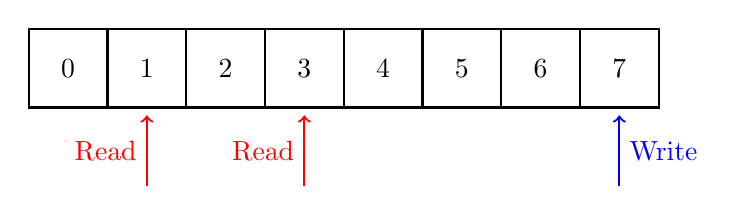
\begin{tikzpicture}
\foreach \i in {0,1,2,3,4,5,6,7} {
    \draw[thick] (\i,0) rectangle (\i+1,1); % Draw each spot in the queue
    \node at (\i+0.5, 0.5) {\i}; % Label each spot
}
\draw[thick, ->, red] (1.5, -1) -- (1.5, -0.1) node[midway, left] {Read};
\draw[thick, ->, red] (3.5, -1) -- (3.5, -0.1) node[midway, left] {Read}; % Added read pointer at position 3
\draw[thick, ->, blue] (7.5, -1) -- (7.5, -0.1) node[midway, right] {Write};
\end{tikzpicture}
\end{center}

An SPMC queue can be tricky to get right. There are many things to consider:
\begin{itemize}
    \item Readers can lapse each other.
    \item Readers can compete for read indices.
    \item Readers can lapse writer.
    \item One reader can starve other readers.
    \item A slow reader can block the system.
\end{itemize}

And under all circumstances, system \textit{correctness} must be maintained.

\section{Design}

For the design:
\begin{itemize}
    \item SPMC is implemented as a circular queue with size of N
    \item The status of individual index is represented as a status array of size N
    \item The status of each index is either UNUSED, WRITTEN, or READING
    \item Each reader maintain its own read pointer
    \item A \textit{outstanding} counter is incremented by the writer when write is complete, 
    and decremented by the reader when it reserves a read
\end{itemize}

Whenever the write finishes a write, it increments \textit{outstanding} to
indicate some buffer is ready to read.\newline 

To read, a reader performs a two-step reservation: 
\begin{itemize}
    \item The reader decrements \textit{outstanding}. A successful decrement means
    the reader is \textit{guaranteed} a read index.
    \item After successful decrement of \textit{outstanding}, the reader walk
    its read pointer until it successfully reserve the next available index to
    read. This is done by attempting to CAS update an index from \textit{WRITTEN} to
    \textit{READING}. If the update fails, then the index was already reserved by another 
    reader.
\end{itemize}

There may be more than one approach in implementing SPMC, the above description
is what we will implement in this chapter.

\section{Spec}

The following is the core reader implementation:
\newline
\begin{pcal}
procedure reader() 
variable 
    i = self;
begin
r_chk_empty:        
    if outstanding # 0 then 
        outstanding := outstanding - 1; 
    else 
    r_early_ret:            
        return;
    end if;
r_try_lock:         
    if status[rptr[i]] = WRITTEN then 
        status[rptr[i]] := READING;
    else 
    r_retry:                
        rptr[i] := (rptr[i] + 1) % N;
            goto r_try_lock;
    end if;
r_data_chk:         
    assert buffer[rptr[i]] = rptr[i] + 1000;
r_read_buf:         
    buffer[rptr[i]] := 0;
r_unlock:           
    status[rptr[i]] := UNUSED;
r_done:             
    return;
end procedure; 
\end{pcal}
\begin{tlatex}
\@x{ {\p@procedure} reader {\p@lparen} {\p@rparen}}%
\@x{ {\p@variable}}%
\@x{\@s{16.4} i \.{=} self {\p@semicolon}}%
\@x{ {\p@begin}}%
\@x{ r\_chk\_empty\@s{.5}\textrm{:}\@s{3}}%
\@x{\@s{16.4} {\p@if} outstanding \.{\neq} 0 {\p@then}}%
\@x{\@s{20.5} outstanding \.{:=} outstanding \.{-} 1 {\p@semicolon}}%
\@x{\@s{16.4} {\p@else}}%
\@x{\@s{16.4} r\_early\_ret\@s{.5}\textrm{:}\@s{3}}%
\@x{\@s{32.8} {\p@return} {\p@semicolon}}%
\@x{\@s{16.4} {\p@end} {\p@if} {\p@semicolon}}%
\@x{ r\_try\_lock\@s{.5}\textrm{:}\@s{3}}%
\@x{\@s{16.4} {\p@if} status [ rptr [ i ] ] \.{=} WRITTEN {\p@then}}%
\@x{\@s{20.5} status [ rptr [ i ] ] \.{:=} READING {\p@semicolon}}%
\@x{\@s{16.4} {\p@else}}%
\@x{\@s{16.4} r\_retry\@s{.5}\textrm{:}\@s{3}}%
 \@x{\@s{32.8} rptr [ i ] \.{:=} ( rptr [ i ] \.{+} 1 ) \.{\%} N
 {\p@semicolon}}%
\@x{\@s{32.8} {\p@goto} r\_try\_lock {\p@semicolon}}%
\@x{\@s{16.4} {\p@end} {\p@if} {\p@semicolon}}%
\@x{ r\_data\_chk\@s{.5}\textrm{:}\@s{3}}%
 \@x{\@s{16.4} {\p@assert} buffer [ rptr [ i ] ] \.{=} rptr [ i ] \.{+} 1000
 {\p@semicolon}}%
\@x{ r\_read\_buf\@s{.5}\textrm{:}\@s{3}}%
\@x{\@s{16.4} buffer [ rptr [ i ] ] \.{:=} 0 {\p@semicolon}}%
\@x{ r\_unlock\@s{.5}\textrm{:}\@s{3}}%
\@x{\@s{16.4} status [ rptr [ i ] ] \.{:=} UNUSED {\p@semicolon}}%
\@x{ r\_done\@s{.5}\textrm{:}\@s{3}}%
\@x{\@s{16.4} {\p@return} {\p@semicolon}}%
\@x{ {\p@end} {\p@procedure} {\p@semicolon}}%
\end{tlatex}
\newline

The reader performs a non-zero check on outstanding. If the outstanding is zero,
the queue is empty, and the reader early returns.\\

If outstanding is K, then at most K readers can reserve an index to read. If system 
has M readers, then M-K readers will fail to reserve a read index. The readers now 
compete to reserve a read. More specifically: 
\begin{itemize}
    \item Reader loads outstanding, stores that onto local variable counter.
    \item Reader early returns if counter is zero 
    \item Reader attempts to update outstanding with CAS using counter and counter - 1.
    \item If CAS fails, go back to the top and retry.
\end{itemize}

If rv is non-success, another reader has \textit{won} the reservation. The
current reader can attempt to reserve again if \textit{outstanding} is
non-zero.\newline

If rv is a success, the reader is \textit{guaranteed} a read. However, readers
may still compete during index reservation. To reserve an index, a reader issues
CAS to update the index status from \textit{WRITTEN} to \textit{READING}. CAS
failure indicates another reader has already reserved this index. The reader
will bump the read pointer and try to reserve the next index.\\

Now let us take a look at the writer implementation:\\

\begin{pcal}
procedure writer() begin
w_chk_full:         
    if outstanding = N - 1 then 
    w_early_ret:            
        return; 
    end if;
w_chk_st:           
    if status[wptr] # UNUSED then 
    w_early_ret2:           
        return;
    end if;
w_write_buf:        
    buffer[wptr] := wptr + 1000;
w_mark_written:     
    status[wptr] := WRITTEN;
w_inc_wptr:         
    wptr := (wptr + 1) % N;
w_inc:              
    outstanding := outstanding + 1;
w_done:             
    return;
end procedure; 
\end{pcal}
\begin{tlatex}
\@x{ {\p@procedure} writer {\p@lparen} {\p@rparen} {\p@begin}}%
\@x{ w\_chk\_full\@s{.5}\textrm{:}\@s{3}}%
\@x{\@s{16.4} {\p@if} outstanding \.{=} N \.{-} 1 {\p@then}}%
\@x{\@s{16.4} w\_early\_ret\@s{.5}\textrm{:}\@s{3}}%
\@x{\@s{32.8} {\p@return} {\p@semicolon}}%
\@x{\@s{16.4} {\p@end} {\p@if} {\p@semicolon}}%
\@x{ w\_chk\_st\@s{.5}\textrm{:}\@s{3}}%
\@x{\@s{16.4} {\p@if} status [ wptr ] \.{\neq} UNUSED {\p@then}}%
\@x{\@s{16.4} w\_early\_ret2\@s{.5}\textrm{:}\@s{3}}%
\@x{\@s{32.8} {\p@return} {\p@semicolon}}%
\@x{\@s{16.4} {\p@end} {\p@if} {\p@semicolon}}%
\@x{ w\_write\_buf\@s{.5}\textrm{:}\@s{3}}%
\@x{\@s{16.4} buffer [ wptr ] \.{:=} wptr \.{+} 1000 {\p@semicolon}}%
\@x{ w\_mark\_written\@s{.5}\textrm{:}\@s{3}}%
\@x{\@s{16.4} status [ wptr ] \.{:=} WRITTEN {\p@semicolon}}%
\@x{ w\_inc\_wptr\@s{.5}\textrm{:}\@s{3}}%
\@x{\@s{16.4} wptr \.{:=} ( wptr \.{+} 1 ) \.{\%} N {\p@semicolon}}%
\@x{ w\_inc\@s{.5}\textrm{:}\@s{3}}%
\@x{\@s{16.4} outstanding \.{:=} outstanding \.{+} 1 {\p@semicolon}}%
\@x{ w\_done\@s{.5}\textrm{:}\@s{3}}%
\@x{\@s{16.4} {\p@return} {\p@semicolon}}%
\@x{ {\p@end} {\p@procedure} {\p@semicolon}}%
\end{tlatex}
\newline

The writer first checks outstanding, and early return if queue is full. After
fullness check, the writer then checks if the current index is UNUSED.  This is
to account for the edge case where a reader has performed the reservation first
step to decrement outstanding but haven't done the actual read. If both checks
pass, then writer now has an \textit{UNUSED} index it can write to.\newline

\section{Safety}

When a reader reserves an index to read, the reader must have exclusive access. 
This can be described as: For any pair of readers inside critical section, they
must operate on different indices:\newline

\begin{tla}
ExclusiveReservation == 
    \A x, y \in READERS: 
        (/\ x /= y 
         /\ pc[x] = "r_read_buf" 
         /\ pc[y] = "r_read_buf") 
            => (rptr[x] # rptr[y])
\end{tla}
\begin{tlatex}
\@x{ ExclusiveReservation \.{\defeq}}%
\@x{\@s{16.4} \A\, x ,\, y \.{\in} READERS \.{:}}%
\@x{\@s{16.4} ( \.{\land} x \.{\neq} y}%
\@x{\@s{20.5} \.{\land} pc [ x ] \.{=}\@w{r\_read\_buf}}%
\@x{\@s{20.5} \.{\land} pc [ y ] \.{=}\@w{r\_read\_buf} )}%
\@x{\@s{20.5} \.{\implies} ( rptr [ x ] \.{\neq} rptr [ y ] )}%
\end{tlatex}
\newline

Similarly, for any reader and writer inside critical section, they must operate
on different indices as well:\newline
\begin{tla}
ExclusiveReadWrite == 
    \A x \in READERS: 
        (/\ pc[x] = "r_read_buf" 
         /\ pc[WRITER] = "w_write_buf") 
            => (rptr[x] # wptr)
\end{tla}
\begin{tlatex}
\@x{ ExclusiveReadWrite \.{\defeq}}%
\@x{\@s{16.4} \A\, x \.{\in} READERS \.{:}}%
\@x{\@s{20.5} ( \.{\land} pc [ x ] \.{=}\@w{r\_read\_buf}}%
\@x{\@s{24.6} \.{\land} pc [ WRITER ] \.{=}\@w{w\_write\_buf} )}%
\@x{\@s{24.6} \.{\implies} ( rptr [ x ] \.{\neq} wptr )}%
\end{tlatex}

\section{Liveness}

All indices must be used as the system runs. The following verifies all unused
indices are eventually used, and all used indicies are eventually unused:
\newline
\begin{tla}
Liveness ==
    /\ \A k \in 0..N-1:
        buffer[k] = 0 ~> buffer[k] # 0
    /\ \A k \in 0..N-1:
        buffer[k] # 0 ~> buffer[k] = 0
\end{tla}
\begin{tlatex}
\@x{ Liveness \.{\defeq}}%
\@x{\@s{16.4} \.{\land} \A\, k \.{\in} 0 \.{\dotdot} N \.{-} 1 \.{:}}%
\@x{\@s{20.5} buffer [ k ] \.{=} 0 \.{\leadsto} buffer [ k ] \.{\neq} 0}%
\@x{\@s{16.4} \.{\land} \A\, k \.{\in} 0 \.{\dotdot} N \.{-} 1 \.{:}}%
\@x{\@s{20.5} buffer [ k ] \.{\neq} 0 \.{\leadsto} buffer [ k ] \.{=} 0}%
\end{tlatex}
\newline

The following describes a more subtle scenario. We need to ensure the system
remains functional even if readers complete out-of-order. The following describe
such scenario, where two non-contiguous indicies have been reserved for reading.
In this case we expect the indicies to eventually be re-used. This means the
system remains functional after such scenario.\newline

\begin{tla}
Liveness2 == 
    \A k \in 0..N-3:
    /\ (/\ status[k] = READING 
        /\ status[k+1] = UNUSED 
        /\ status[k+2] = READING)
        ~> (status[k] = WRITTEN)
    /\ (/\ status[k] = READING 
        /\ status[k+1] = UNUSED 
        /\ status[k+2] = READING)
        ~> (status[k+2] = WRITTEN)
\end{tla}
\begin{tlatex}
\@x{ Liveness2 \.{\defeq}}%
\@x{\@s{16.4} \A\, k \.{\in} 0 \.{\dotdot} N \.{-} 3 \.{:}}%
\@x{\@s{16.4} \.{\land} ( \.{\land} status [ k ] \.{=} READING}%
\@x{\@s{20.5} \.{\land} status [ k \.{+} 1 ] \.{=} UNUSED}%
\@x{\@s{20.5} \.{\land} status [ k \.{+} 2 ] \.{=} READING )}%
\@x{\@s{20.5} \.{\leadsto} ( status [ k ] \.{=} WRITTEN )}%
\@x{\@s{16.4} \.{\land} ( \.{\land} status [ k ] \.{=} READING}%
\@x{\@s{20.5} \.{\land} status [ k \.{+} 1 ] \.{=} UNUSED}%
\@x{\@s{20.5} \.{\land} status [ k \.{+} 2 ] \.{=} READING )}%
\@x{\@s{20.5} \.{\leadsto} ( status [ k \.{+} 2 ] \.{=} WRITTEN )}%
\end{tlatex}

% \end{document}
